% Options for packages loaded elsewhere
\PassOptionsToPackage{unicode}{hyperref}
\PassOptionsToPackage{hyphens}{url}
%
\documentclass[
  man]{apa6}
\usepackage{amsmath,amssymb}
\usepackage{iftex}
\ifPDFTeX
  \usepackage[T1]{fontenc}
  \usepackage[utf8]{inputenc}
  \usepackage{textcomp} % provide euro and other symbols
\else % if luatex or xetex
  \usepackage{unicode-math} % this also loads fontspec
  \defaultfontfeatures{Scale=MatchLowercase}
  \defaultfontfeatures[\rmfamily]{Ligatures=TeX,Scale=1}
\fi
\usepackage{lmodern}
\ifPDFTeX\else
  % xetex/luatex font selection
\fi
% Use upquote if available, for straight quotes in verbatim environments
\IfFileExists{upquote.sty}{\usepackage{upquote}}{}
\IfFileExists{microtype.sty}{% use microtype if available
  \usepackage[]{microtype}
  \UseMicrotypeSet[protrusion]{basicmath} % disable protrusion for tt fonts
}{}
\makeatletter
\@ifundefined{KOMAClassName}{% if non-KOMA class
  \IfFileExists{parskip.sty}{%
    \usepackage{parskip}
  }{% else
    \setlength{\parindent}{0pt}
    \setlength{\parskip}{6pt plus 2pt minus 1pt}}
}{% if KOMA class
  \KOMAoptions{parskip=half}}
\makeatother
\usepackage{xcolor}
\usepackage{graphicx}
\makeatletter
\def\maxwidth{\ifdim\Gin@nat@width>\linewidth\linewidth\else\Gin@nat@width\fi}
\def\maxheight{\ifdim\Gin@nat@height>\textheight\textheight\else\Gin@nat@height\fi}
\makeatother
% Scale images if necessary, so that they will not overflow the page
% margins by default, and it is still possible to overwrite the defaults
% using explicit options in \includegraphics[width, height, ...]{}
\setkeys{Gin}{width=\maxwidth,height=\maxheight,keepaspectratio}
% Set default figure placement to htbp
\makeatletter
\def\fps@figure{htbp}
\makeatother
\setlength{\emergencystretch}{3em} % prevent overfull lines
\providecommand{\tightlist}{%
  \setlength{\itemsep}{0pt}\setlength{\parskip}{0pt}}
\setcounter{secnumdepth}{-\maxdimen} % remove section numbering
% Make \paragraph and \subparagraph free-standing
\ifx\paragraph\undefined\else
  \let\oldparagraph\paragraph
  \renewcommand{\paragraph}[1]{\oldparagraph{#1}\mbox{}}
\fi
\ifx\subparagraph\undefined\else
  \let\oldsubparagraph\subparagraph
  \renewcommand{\subparagraph}[1]{\oldsubparagraph{#1}\mbox{}}
\fi
\newlength{\cslhangindent}
\setlength{\cslhangindent}{1.5em}
\newlength{\csllabelwidth}
\setlength{\csllabelwidth}{3em}
\newlength{\cslentryspacingunit} % times entry-spacing
\setlength{\cslentryspacingunit}{\parskip}
\newenvironment{CSLReferences}[2] % #1 hanging-ident, #2 entry spacing
 {% don't indent paragraphs
  \setlength{\parindent}{0pt}
  % turn on hanging indent if param 1 is 1
  \ifodd #1
  \let\oldpar\par
  \def\par{\hangindent=\cslhangindent\oldpar}
  \fi
  % set entry spacing
  \setlength{\parskip}{#2\cslentryspacingunit}
 }%
 {}
\usepackage{calc}
\newcommand{\CSLBlock}[1]{#1\hfill\break}
\newcommand{\CSLLeftMargin}[1]{\parbox[t]{\csllabelwidth}{#1}}
\newcommand{\CSLRightInline}[1]{\parbox[t]{\linewidth - \csllabelwidth}{#1}\break}
\newcommand{\CSLIndent}[1]{\hspace{\cslhangindent}#1}
\ifLuaTeX
\usepackage[bidi=basic]{babel}
\else
\usepackage[bidi=default]{babel}
\fi
\babelprovide[main,import]{english}
% get rid of language-specific shorthands (see #6817):
\let\LanguageShortHands\languageshorthands
\def\languageshorthands#1{}
% Manuscript styling
\usepackage{upgreek}
\captionsetup{font=singlespacing,justification=justified}

% Table formatting
\usepackage{longtable}
\usepackage{lscape}
% \usepackage[counterclockwise]{rotating}   % Landscape page setup for large tables
\usepackage{multirow}		% Table styling
\usepackage{tabularx}		% Control Column width
\usepackage[flushleft]{threeparttable}	% Allows for three part tables with a specified notes section
\usepackage{threeparttablex}            % Lets threeparttable work with longtable

% Create new environments so endfloat can handle them
% \newenvironment{ltable}
%   {\begin{landscape}\centering\begin{threeparttable}}
%   {\end{threeparttable}\end{landscape}}
\newenvironment{lltable}{\begin{landscape}\centering\begin{ThreePartTable}}{\end{ThreePartTable}\end{landscape}}

% Enables adjusting longtable caption width to table width
% Solution found at http://golatex.de/longtable-mit-caption-so-breit-wie-die-tabelle-t15767.html
\makeatletter
\newcommand\LastLTentrywidth{1em}
\newlength\longtablewidth
\setlength{\longtablewidth}{1in}
\newcommand{\getlongtablewidth}{\begingroup \ifcsname LT@\roman{LT@tables}\endcsname \global\longtablewidth=0pt \renewcommand{\LT@entry}[2]{\global\advance\longtablewidth by ##2\relax\gdef\LastLTentrywidth{##2}}\@nameuse{LT@\roman{LT@tables}} \fi \endgroup}

% \setlength{\parindent}{0.5in}
% \setlength{\parskip}{0pt plus 0pt minus 0pt}

% Overwrite redefinition of paragraph and subparagraph by the default LaTeX template
% See https://github.com/crsh/papaja/issues/292
\makeatletter
\renewcommand{\paragraph}{\@startsection{paragraph}{4}{\parindent}%
  {0\baselineskip \@plus 0.2ex \@minus 0.2ex}%
  {-1em}%
  {\normalfont\normalsize\bfseries\itshape\typesectitle}}

\renewcommand{\subparagraph}[1]{\@startsection{subparagraph}{5}{1em}%
  {0\baselineskip \@plus 0.2ex \@minus 0.2ex}%
  {-\z@\relax}%
  {\normalfont\normalsize\itshape\hspace{\parindent}{#1}\textit{\addperi}}{\relax}}
\makeatother

\makeatletter
\usepackage{etoolbox}
\patchcmd{\maketitle}
  {\section{\normalfont\normalsize\abstractname}}
  {\section*{\normalfont\normalsize\abstractname}}
  {}{\typeout{Failed to patch abstract.}}
\patchcmd{\maketitle}
  {\section{\protect\normalfont{\@title}}}
  {\section*{\protect\normalfont{\@title}}}
  {}{\typeout{Failed to patch title.}}
\makeatother

\usepackage{xpatch}
\makeatletter
\xapptocmd\appendix
  {\xapptocmd\section
    {\addcontentsline{toc}{section}{\appendixname\ifoneappendix\else~\theappendix\fi\\: #1}}
    {}{\InnerPatchFailed}%
  }
{}{\PatchFailed}
\keywords{Open Data, Attentional Control, SQL\newline\indent Word count: X}
\DeclareDelayedFloatFlavor{ThreePartTable}{table}
\DeclareDelayedFloatFlavor{lltable}{table}
\DeclareDelayedFloatFlavor*{longtable}{table}
\makeatletter
\renewcommand{\efloat@iwrite}[1]{\immediate\expandafter\protected@write\csname efloat@post#1\endcsname{}}
\makeatother
\usepackage{lineno}

\linenumbers
\usepackage{csquotes}
\usepackage{mathrsfs}
\usepackage[makeroom]{cancel}
\usepackage{pcl}
\usepackage{setspace}\doublespacing
\usepackage{marginnote}
\newcommand{\readme}[1]{\emph{\marginnote{Julia} (#1)}}
\usepackage{pifont}
\usepackage{hyperref}
\usepackage{colortbl}
\hypersetup{colorlinks=true,urlcolor=blue,citecolor=black,linkcolor=black}
\ifLuaTeX
  \usepackage{selnolig}  % disable illegal ligatures
\fi
\IfFileExists{bookmark.sty}{\usepackage{bookmark}}{\usepackage{hyperref}}
\IfFileExists{xurl.sty}{\usepackage{xurl}}{} % add URL line breaks if available
\urlstyle{same}
\hypersetup{
  pdftitle={Attentional Control Data Collection: A Resource for Efficient Data Reuse},
  pdfauthor={Julia M. Haaf1, Madlen Hoffstadt1, \& Sven Lesche2},
  pdflang={en-EN},
  pdfkeywords={Open Data, Attentional Control, SQL},
  hidelinks,
  pdfcreator={LaTeX via pandoc}}

\title{Attentional Control Data Collection: A Resource for Efficient Data Reuse}
\author{Julia M. Haaf\textsuperscript{1}, Madlen Hoffstadt\textsuperscript{1}, \& Sven Lesche\textsuperscript{2}}
\date{}


\shorttitle{Attentional Control Data Collection}

\authornote{

We are indepted to Arte Bischop for her thesis work on the initial SQL data base.

This work was supported in part by a Veni grant from the NWO (VI.Veni.201G.019) and a talent grant by Amsterdam Brain \& Cognition (ABC.T09.0921) to J.M.H.

The authors made the following contributions. Julia M. Haaf: Conceptualization, Writing - Original Draft Preparation, Writing - Review \& Editing; Madlen Hoffstadt: Conceptualization, Writing - Original Draft Preparation, Writing - Review \& Editing; Sven Lesche: Conceptualization, Writing - Original Draft Preparation, Writing - Review \& Editing.

Correspondence concerning this article should be addressed to Julia M. Haaf, Nieuwe Achtergracht 129B, 1018 WT Amsterdam, The Netherlands.. E-mail: \href{mailto:j.m.haaf@uva.nl}{\nolinkurl{j.m.haaf@uva.nl}}

}

\affiliation{\vspace{0.5cm}\textsuperscript{1} University of Amsterdam\\\textsuperscript{2} University of Heidelberg}

\note{Version 1, October 2023}

\abstract{%
One or two sentences providing a \textbf{basic introduction} to the field, comprehensible to a scientist in any discipline.

Two to three sentences of \textbf{more detailed background}, comprehensible to scientists in related disciplines.

One sentence clearly stating the \textbf{general problem} being addressed by this particular study.

One sentence summarizing the main result (with the words ``\textbf{here we show}'' or their equivalent).

Two or three sentences explaining what the \textbf{main result} reveals in direct comparison to what was thought to be the case previously, or how the main result adds to previous knowledge.

One or two sentences to put the results into a more \textbf{general context}.

Two or three sentences to provide a \textbf{broader perspective}, readily comprehensible to a scientist in any discipline.
}



\begin{document}
\maketitle

Making data openly available has been a central demand by reformers since the start of the reproducibility crisis in psychology {[}REFS{]}. Fortunately, this demand has lead to a considerable increase in data availability. While only about 25\% of data were shared after request in 2006 (Wicherts, Borsboom, Kats, \& Molenaar, 2006), publicly sharing data upon publication is now more and more the norm. This cultural shift is also increasingly institutionalized. Universities and funding agencies prioritize open data, and some journals even mandate the publication of data with every published article (Sloman, 2015). In addition, technology like the Open Science Framework (OSF) and other data sharing facilities enable an easy process for researchers, further reducing barriers to share data.

Data sharing serves two goals: 1. To make the scientific process more transparent and enable error and fraud detection, and 2. to make the scientific process more efficient by allowing data reuse for different research projects. Current data sharing efforts, however, seemingly focus overwhelmingly on the first goal {[}REF Cruewell et al, 2023{]}. Whenever researchers complying with common data sharing procedures publish an article, they share the corresponding data on the OSF, ideally in a format that allows to redo the exact analyses reported in the article. The OSF repository is linked in the article, and readers may access the data through this link and check whether analysis code and shared data correspond to the results section in the article. This setup, while appropriate for the first goal of data sharing, ignores the second goal of data reuse.

To enable data reuse, data sharing needs to be approached differently. For example, consider a researcher (like the first author of the current paper) might me interested in the Stroop task (Stroop, 1935). The Stroop task is popular in cognitive psychology (MacLeod, 1991), so we may assume that many studies include this or similar tasks in their studies. Instead of running yet another Stroop experiment, the researcher decides to use existing data to explore their research question before designing a more targeted study. First, the researcher needs to be able to find open Stroop task data. Currently, they could either search for papers on the topic and check whether open data are provided, or search directly via OSF or other data sharing servers. However, neither of these options is very promising as the vast majority of articles in the literature does not provide raw data and data sharing servers are not equipped with sufficient search options. Second, data sets need to be accessed easily and in a general, understandable format ready for reuse. There are data sharing formats that provide this structure {[}REF{]}, but they are rarely used. Additionally, data are usually shared on the level necessary for the original analysis. In case of the Stroop task, shared data might provide the Stroop effect per participant, but for this new analysis the researcher needs trial-level data. So again, there is yet another barrier for data reuse.

We think it is necessary to provide a data sharing solution that solves the current problems and enables easy and efficient data reuse. Here, we propose to gather open data sets from a specific research area in an SQL data base. This process requires little to no work in addition to current data sharing policies from the authors of original papers, some work from the lab(s) setting up the data base, and little to no work from the researchers who wish to reuse open data. We describe the process and structure we used to set up a data base of attentional control tasks called the Attentional Control Data Collection (ACDC). The data base includes XXX data sets from XXX publications from tasks like the Stroop, Simon, and flanker tasks. Subsequently, we show how the data can be explored using a Shiny app and accessed using an R-package. In an example analysis, we assess the reliability of the included tasks. This section highlights how an open data base like ACDC can aid meta-analytic efforts as well as methodological innovation.

To provide a little history of the project, the Attentional Control Data Collection was inspired by a collection of open data sets from attentional control tasks by the Perception and Cognition Lab led by J. Rouder (\href{https://github.com/PerceptionCognitionLab/data0}{url}). Colleagues provided the first author and Rouder with data sets for their statistical work (Haaf \& Rouder, 2017; \textbf{Rouder:etal:2023?}). To ensure that data sets were accessible, we gathered them in a github repository. However, there was little structure to the collection, and github repositories are neither stable entities nor are they designed as data storage. Here, we describe how a structured data collection can be achieved and which benefits it provides.

\hypertarget{sqlight-data-base}{%
\section{SQLight Data Base}\label{sqlight-data-base}}

One of the most standard ways in computer science for storing data is using SQL data bases. Structured query language (SQL) allows to create, access and manipulate a structured data storage. SQL data bases consist of data tables and relations between these tables. There are many flavors of SQL data bases. Here, we decided to use an SQLight data base, a lightweight solution that allows us to store the entire data base in a single file of moderate size that can be downloaded by researchers for data reuse. In this section we describe the structure of the data base and the data currently included. Researchers who simply want to use ACDC may safely skip this section.

\hypertarget{data-base-structure}{%
\subsection{Data Base Structure}\label{data-base-structure}}

\begin{itemize}
\tightlist
\item
  SQL databases are composed of several data tables consisting of rows and columns.

  \begin{itemize}
  \tightlist
  \item
    Each row in a data table has foreign key (essentially a row ID) which uniquely identifies it. Additionally, SQL data tables may contain foreign keys which reference a unique row in another data table. In contrast to primary keys, these foreign keys allow for duplicate values within the same data table.
  \item
    For instance, a study table may store information about all studies in a database where each row corresponds to one study. Here the foreign key is the study\_id. We can ensure that our database links each study to the publication it was published in by adding a foreign key called publication\_id which references the unique identifier of the respective publication in a publication table (see Figure 1).
  \end{itemize}
\end{itemize}



\begin{figure}
\centering
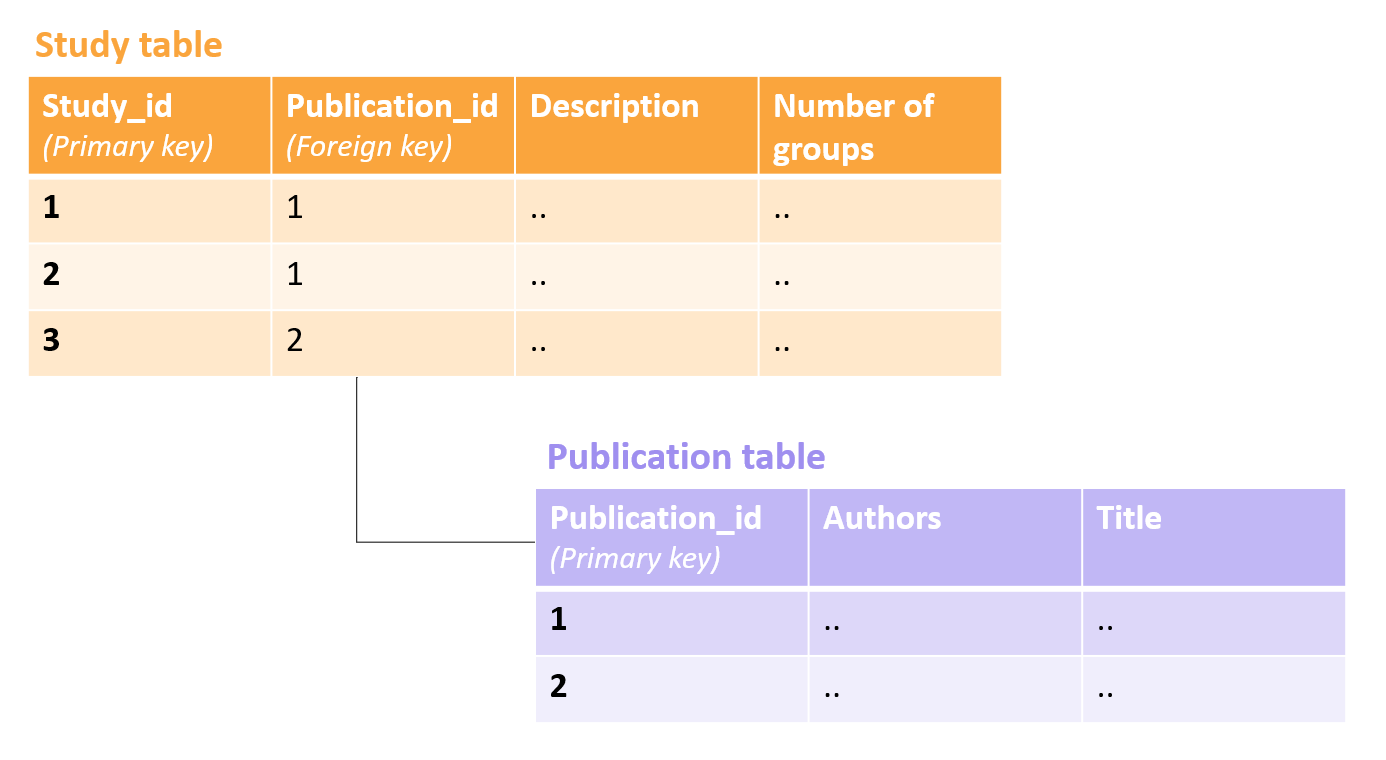
\includegraphics{images/illustrate_SQL_keys.png}
\caption{(\#fig:figure 1)Figure 1. Illustrative example of using foreign and primary keys in a SQL database.}
\end{figure}

\begin{itemize}
\tightlist
\item
  The structure of ACDC is adapted to the logic of publications consisting of one or multiple studies which in turn include one or several datasets (see Figure 2).

  \begin{itemize}
  \tightlist
  \item
    Each dataset stores information about a single attentional control task within a certain study. A dataset table stores information about each dataset (such as sample size) while the observation table contains the actual attentional control task data.
  \item
    A between table contains information about between-person manipulations on a study level and a within table stores information about within-person manipulations within a dataset.
  \item
    Note that since the congruency between stimuli is part of every attentional control task it is not considered a within-manipulation in this database but is per default included in the observation table.
  \item
    The combination of within- and between-manipulations results in several possible conditions within a dataset, which are stored in a condition table.

    \begin{itemize}
    \item
      \begin{itemize}
      \tightlist
      \item
        Add this?: Both the condition table and the observation table contain the within\_id, between\_id and condition\_id. We deliberately chose this duplication within our database to increase the speed of accessing data through our R package and through the R shiny app.
      \end{itemize}
    \end{itemize}
  \end{itemize}
\end{itemize}



\begin{figure}
\centering
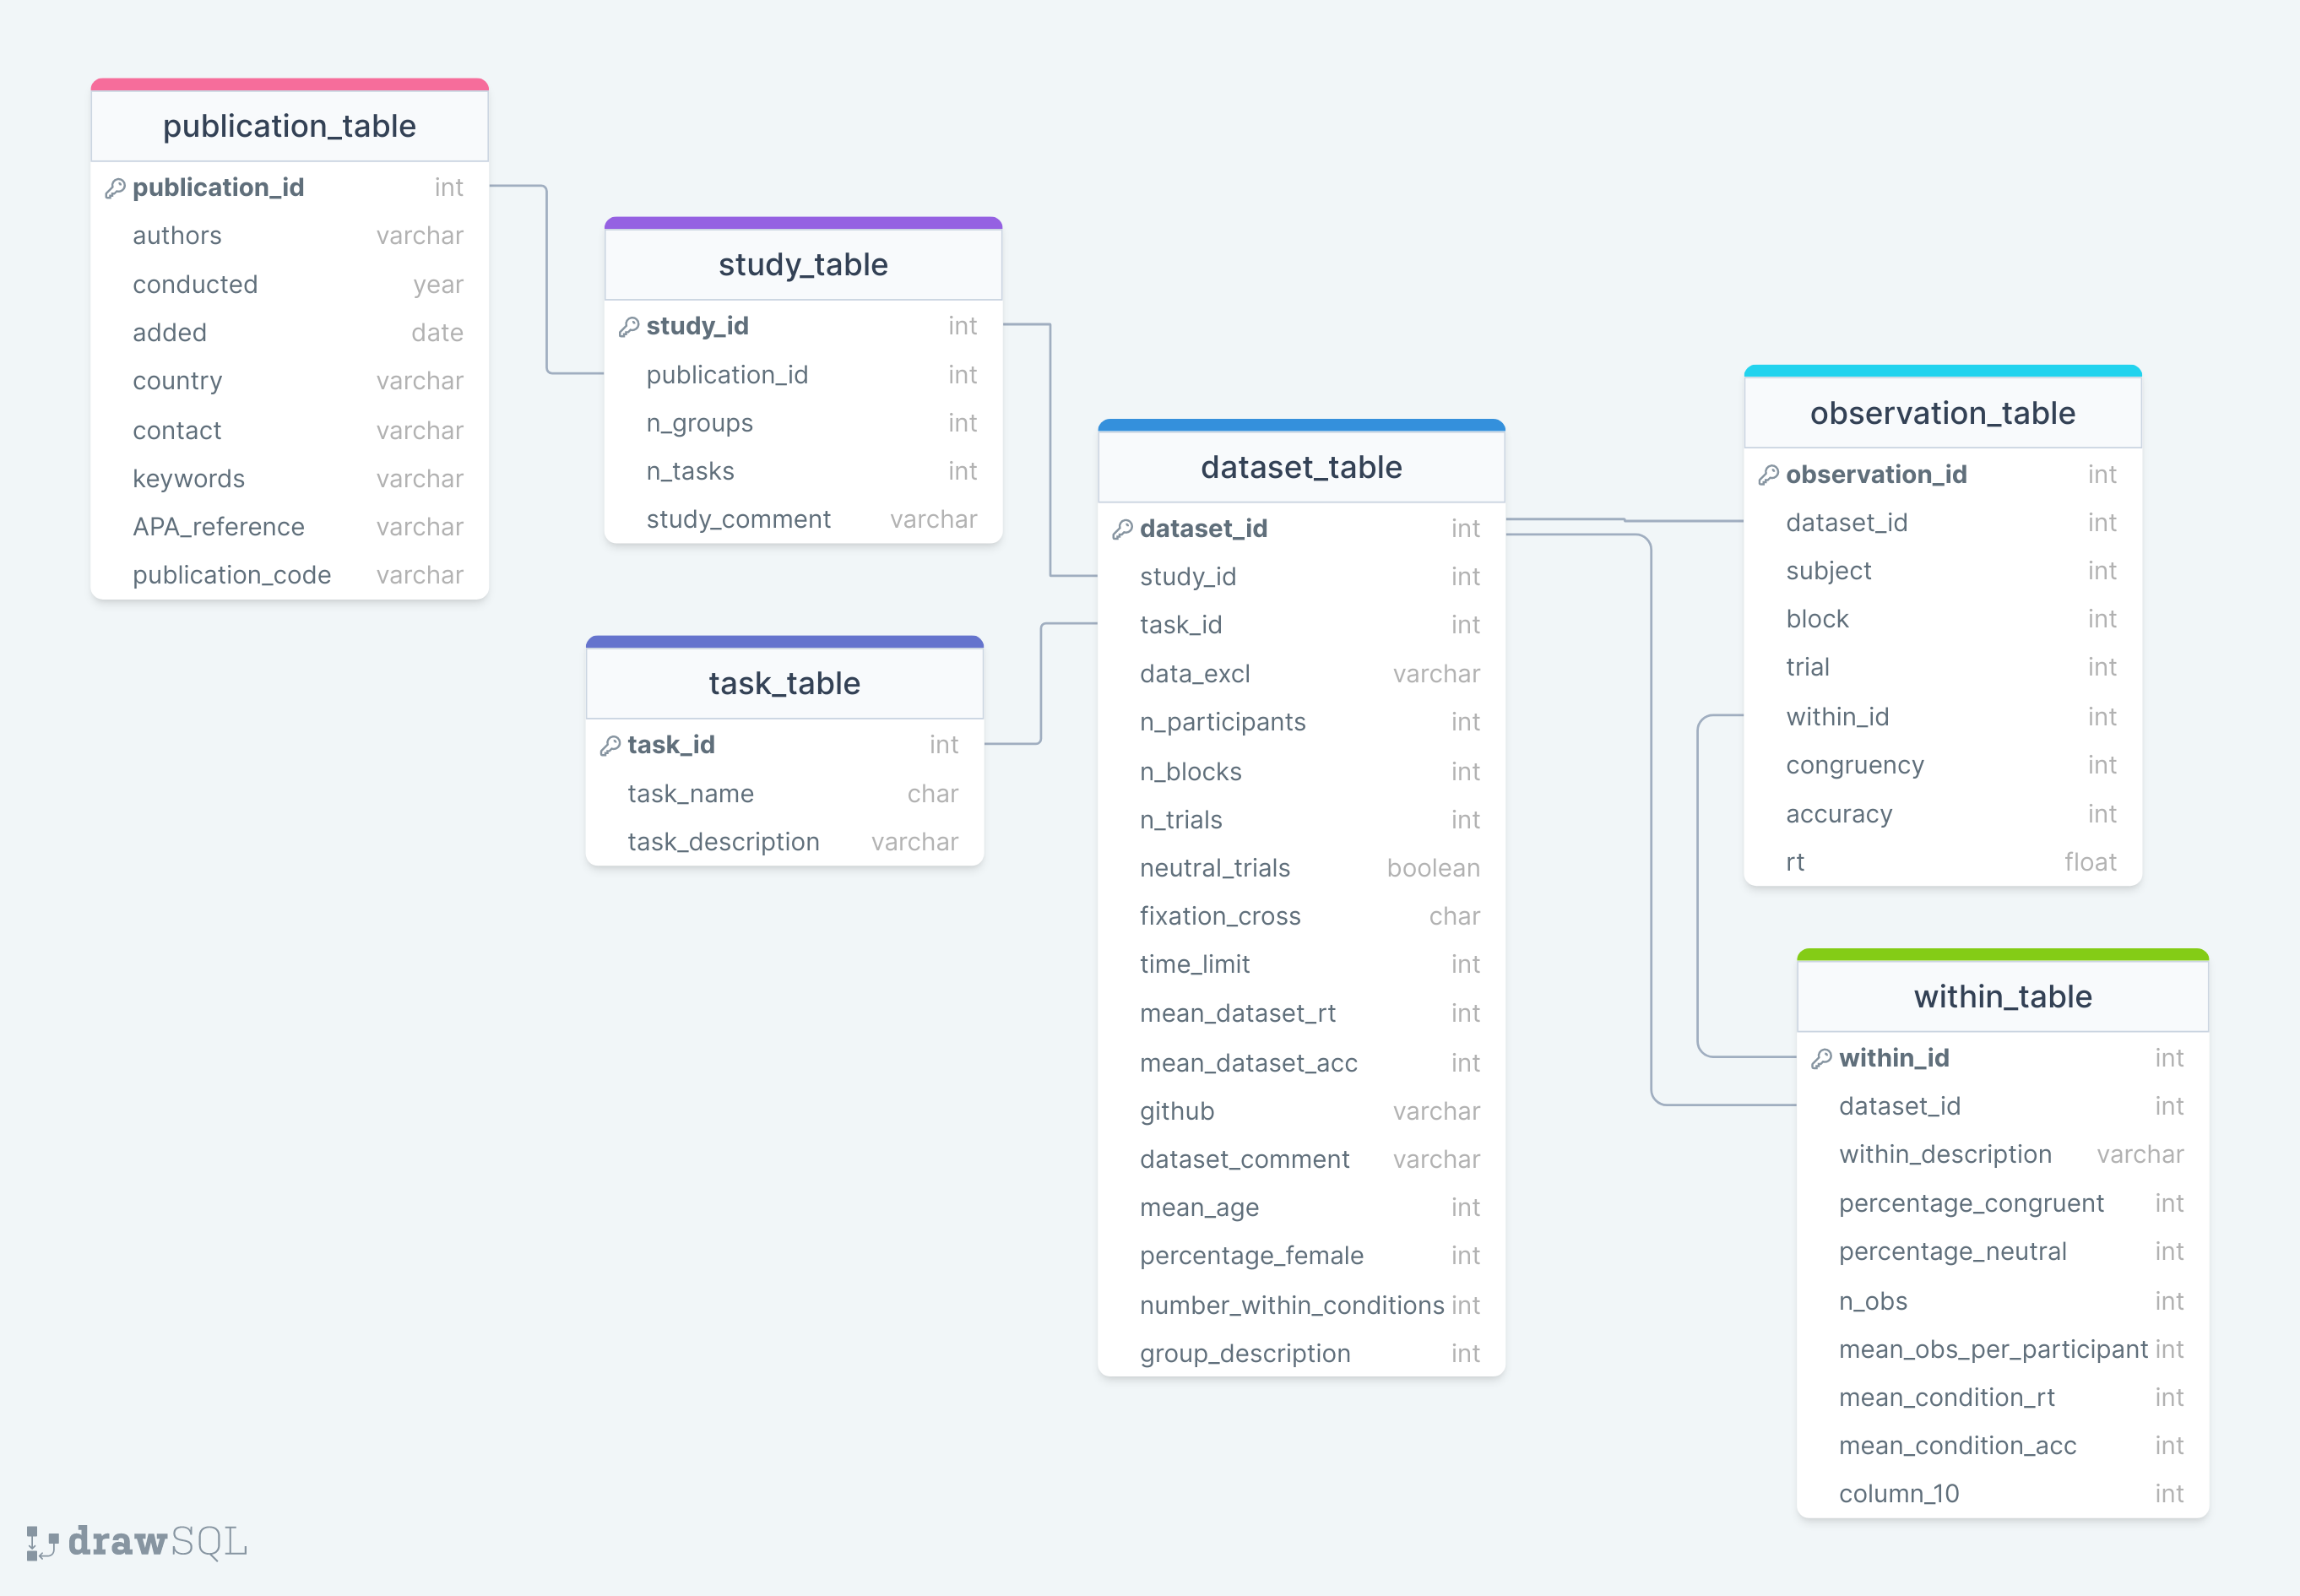
\includegraphics{images/db_structure.png}
\caption{(\#fig:figure 2)Figure 2. Structure of the ACDC database. Note. Primary keys are indicated by the key symbol. References between data tables are illustrated through lines connecting columns across data tables. This overview includes the data type of each column: integers (int), numbers with decimal places (float), characters (varchar) and logical true/false values (Booleans).}
\end{figure}

\hypertarget{included-data}{%
\subsection{Included Data}\label{included-data}}

\hypertarget{accessing-the-data-base}{%
\section{Accessing the Data Base}\label{accessing-the-data-base}}

\hypertarget{shiny-app}{%
\subsection{Shiny App}\label{shiny-app}}

\hypertarget{r-package}{%
\subsection{R-Package}\label{r-package}}

\hypertarget{queries-and-output}{%
\subsection{Queries and Output}\label{queries-and-output}}

\hypertarget{example-analysis}{%
\section{Example Analysis}\label{example-analysis}}

\hypertarget{reliability-of-experimental-tasks}{%
\subsection{Reliability of Experimental Tasks}\label{reliability-of-experimental-tasks}}

\hypertarget{a-closer-look-at-the-stroop-task}{%
\subsection{A Closer Look at the Stroop Task}\label{a-closer-look-at-the-stroop-task}}

\hypertarget{discussion}{%
\section{Discussion}\label{discussion}}

\newpage

\hypertarget{references}{%
\section{References}\label{references}}

\hypertarget{refs}{}
\begin{CSLReferences}{1}{0}
\leavevmode\vadjust pre{\hypertarget{ref-Haaf:Rouder:2017}{}}%
Haaf, J. M., \& Rouder, J. N. (2017). Developing constraint in {B}ayesian mixed models. \emph{Psychological Methods}, \emph{22}(4), 779--798.

\leavevmode\vadjust pre{\hypertarget{ref-MacLeod:1991}{}}%
MacLeod, C. (1991). Half a century of research on the {S}troop effect: {A}n integrative review. \emph{Psychological Bulletin}, \emph{109}, 163--203.

\leavevmode\vadjust pre{\hypertarget{ref-Sloman:2015}{}}%
Sloman, S. A. (2015). Opening editorial: The changing face of cognition. \emph{Cognition}, \emph{135}, 1--3.

\leavevmode\vadjust pre{\hypertarget{ref-Stroop:1935}{}}%
Stroop, J. R. (1935). Studies of interference in serial verbal reactions. \emph{Journal of Experimental Psychology}, \emph{18}, 643--662.

\leavevmode\vadjust pre{\hypertarget{ref-Wicherts:etal:2006}{}}%
Wicherts, J. M., Borsboom, D., Kats, J., \& Molenaar, D. (2006). The poor availability of psychological research data for reanalysis. \emph{American Psychologist}, \emph{61}(7), 726--728. Retrieved from \url{http://wicherts.socsci.uva.nl/datasharing.pdf}

\end{CSLReferences}


\end{document}
